\documentclass[USenglish]{article}
\usepackage[utf8]{inputenc}
\usepackage[big,online]{dgruyter}
\usepackage{lmodern}
\usepackage{microtype}
\usepackage[numbers,square,sort&compress]{natbib}
\usepackage{amsmath,amssymb}
\usepackage{booktabs}
\usepackage{tabularx}
\usepackage{ragged2e}
\usepackage{array}
\usepackage{siunitx}
\usepackage{graphicx}
\usepackage{url}
\usepackage{rotating}
\newcolumntype{C}[1]{>{\centering\arraybackslash}m{#1}}
\newcolumntype{M}[1]{>{\RaggedRight\arraybackslash}m{#1}}

\begin{document}

\articletype{Research Article}
\journalname{Frequenz}

\title{Genetic-algorithm-optimized spline patch antenna with a PTFE photonic band-gap substrate for 0.35 THz applications}
\runningtitle{GA-optimized spline THz patch antenna}
\author*[1]{Djalal Ziani-Kerarti}
\author[2]{Fatima Zohra Marouf}
\runningauthor{D. Ziani-Kerarti and F. Z. Marouf}
\affil[1]{\protect\raggedright Department of Specialization and Post-Graduation, National Higher School of Telecommunications and ICT, LaRATIC Laboratory, Es-Senia, Oran, Algeria, e-mail: djalal.zianikerarti@ensttic.dz}
\affil[2]{\protect\raggedright Department of Electrical Engineering, National Polytechnic School of Oran, LAAS Laboratory, Es-Senia, Oran, Algeria}

\abstract{The terahertz frequency range offers broad bandwidth for future short-range wireless links but places stringent demands on antenna matching and radiation efficiency. This study presents a compact single-element microstrip patch antenna for the 0.35 THz atmospheric transmission window. The radiating contour is defined by a quadratic spline whose control points are optimized with a genetic algorithm. A photonic band-gap lattice of cylindrical air holes is integrated into a polytetrafluoroethylene substrate to reduce surface-wave transmission near the operating frequency. Full-wave simulations are performed independently in CST Microwave Studio using the finite integration technique and in ANSYS HFSS using the finite element method. The PBG design produces a simulated S11 minimum of -44.65 dB at 0.35 THz in CST and approximately -26.28 dB near 0.344 THz in HFSS. Its simulated -10 dB impedance bandwidth is 56.42 GHz, with a peak gain of 7.22 dBi and a radiation efficiency of 93.56\%. The results support the use of spline geometry and substrate-level PBG engineering as a compact single-element approach for THz antenna research.}
\keywords{terahertz antenna; microstrip patch; photonic band gap; antenna efficiency; genetic algorithm; PTFE}

\maketitle

\section{Introduction}
The terahertz (THz) frequency band is an important candidate for next-generation wireless communication systems, particularly within emerging 6G research~\cite{strinati_6g_2019,he_overview_2020}. An exponential growth in connected devices and data consumption has created an urgent demand for higher data rates and more reliable connections, pushing researchers to explore technologies that leverage the vast bandwidth of the THz spectrum to overcome the limitations of current millimeter-wave and sub-THz systems~\cite{jamshed_antenna_2020,hajiyat_antenna_2021}.

This technological shift could support the proliferation of connected devices and enable data-intensive applications such as augmented reality, holographic communications, ultra-high-definition video streaming, and massive Internet of Things (IoT) deployments~\cite{jornet_internet_2012,amin_step_2022}. The enormous bandwidth available at THz frequencies---often reaching 10\% of the carrier frequency---is highly attractive for high-data-rate communications and advanced sensing~\cite{sen_physical_2022}. Furthermore, the unique properties of THz waves, including their ability to interact with molecular resonances and their high spatial resolution, open new possibilities for imaging, spectroscopy, security screening, and short-range high-capacity links~\cite{nissanov_terahertz_2023,krishna_rhombus_2021}.

Despite these advantages, integrating THz technology into wireless infrastructures presents significant challenges. At such high frequencies, device miniaturization, fabrication tolerances, and material losses become critical bottlenecks, and antennas must simultaneously achieve high gain, high radiation efficiency, and wide impedance bandwidth within compact footprints~\cite{ullah_thz_2019}. Emerging materials such as graphene and metamaterials have enabled reconfigurable and wideband THz platforms by exploiting tunable surface conductivity and engineered resonances~\cite{moradi_graphene_2021,krishna_graphene_2023}. However, many of these solutions involve complex multilayer structures, biasing networks, or advanced fabrication processes that can limit scalability and increase fabrication complexity.

Recent advances in THz antenna design thus explore two complementary directions: (i) geometry-driven optimization of planar radiators, including spline- and Bézier-shaped patches for super-wideband operation~\cite{marouf_bezier_2023}, and (ii) substrate and environment engineering using periodic structures such as photonic band-gap (PBG) lattices, defected ground structures (DGS), and metamaterial inclusions~\cite{khezzar_pbg_2021,ullah_thz_2019,temmar_bspo_2019,devapriya_metamaterial_2019}. For terrestrial links, the atmospheric transmission window around 0.35~THz is particularly compelling, as it offers a crucial balance between wide available bandwidth and relatively low atmospheric attenuation, which may be suitable for short-to-medium-range communication in future 6G systems~\cite{strinati_6g_2019,khezzar_pbg_2021}.

In this context, antenna elements suitable for array and MIMO architectures at sub-THz and THz frequencies have attracted considerable attention~\cite{mousa_ebg_2026,li_triband_2024,nirob_grid_2025}. Several works have proposed multi-port MIMO antennas and compact arrays optimized for isolation, beam steering, and pattern control, often relying on fractal geometries, metamaterials, or regression-based machine-learning models~\cite{panda_fractal_2025,devapriya_metamaterial_2019,krishna_rhombus_2021}. These architectures demonstrate the feasibility of high-capacity THz links but require single-element radiators with balanced gain, bandwidth, and efficiency as building blocks.

Addressing these challenges, this paper presents a design methodology for a microstrip patch antenna operating at 0.35~THz. Our approach combines a genetically optimized, spline-shaped radiating element with a photonic band-gap (PBG) structure integrated into a polytetrafluoroethylene (PTFE) substrate~\cite{john_spline_monopole_2007,khezzar_pbg_2021}. The continuous curvature of the spline radiator is expected to promote a smoother surface-current distribution and reduce abrupt edge effects, while the periodic air-hole lattice in PTFE is designed to create a frequency-selective stopband that can suppress surface-wave propagation near the operating frequency~\cite{temmar_bspo_2019,kushwaha_photonic_2018}. This combination is intended to improve impedance matching, gain, and radiation efficiency for a single-element THz antenna operating in the 0.35~THz atmospheric window.

In contrast to existing PBG-enhanced and optimization-based THz antennas, including recent PSO- and ML-driven designs applied to PBG geometries and array configurations~\cite{babaahmed_hybrid_2025,li_triband_2024,panda_fractal_2025}, the proposed work focuses on jointly optimizing the fundamental radiating geometry and the surrounding PBG substrate to achieve a balanced improvement across S11, bandwidth, gain, and radiation efficiency. Full-wave simulations using CST Microwave Studio and ANSYS HFSS show consistent trends between the two solvers, supporting the use of the spline-based PBG radiator as a potential building block for compact, high-data-rate THz links and future array/MIMO systems envisioned in 6G networks.

This work is distinguished by the following key contributions:
\begin{itemize}
    \item A spline-shaped microstrip radiator optimized via a genetic algorithm at 0.35~THz, providing smooth current distribution and enhanced matching.
    \item A PTFE-based PBG perforated substrate engineered to open a bandgap around 0.35~THz, effectively suppressing surface waves and improving gain and radiation efficiency.
    \item Cross-validated CST/HFSS simulations with quantified deviations in resonant frequency, return loss, bandwidth, gain, and efficiency, providing a numerical consistency check.
    \item A design framework that can be extended towards array/MIMO and machine-learning-assisted optimization of THz antennas, bridging geometric optimization and data-driven modeling.
\end{itemize}


% II. ANTENNA DESIGN AND SIMULATION METHODOLOGY

\section{Antenna Design and Simulation Methodology}
\label{sec:design}

The proposed antenna design follows a multi-stage methodology, illustrated in the flowchart of Figure~\ref{fig:flowchart}. The process begins with geometric modeling of the spline-shaped radiator, followed by shape optimization via a genetic algorithm (GA), substrate selection, performance enhancement through PBG integration, and finally, parametric sensitivity analysis to quantify parameter sensitivity.

\begin{figure}[ht]
\centering
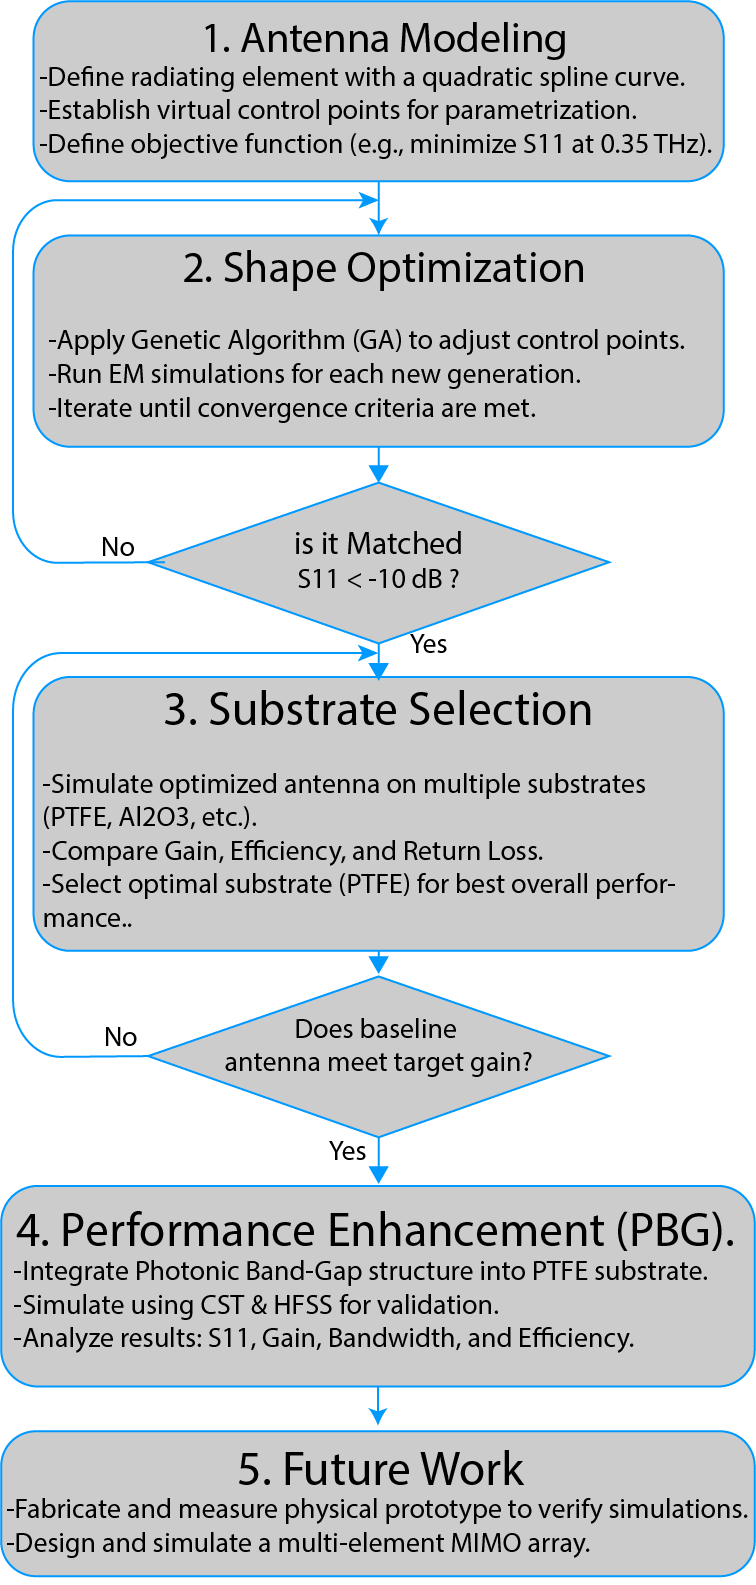
\includegraphics[width=0.7\linewidth]{../../assets/figures/fig1.png}
\caption{Flowchart of the antenna design and optimization methodology, from initial modeling to performance enhancement and parametric sensitivity analysis.}
\label{fig:flowchart}
\end{figure}

\subsection{Radiator and Antenna Geometry}
\label{subsec:radiator}

The core innovation of the antenna is its radiating element, whose profile is defined by a quadratic B-spline curve. This approach avoids the sharp corners typical of conventional rectangular or circular patch antennas and is intended to promote a smoother surface-current distribution and reduce abrupt edge effects. The spline contour is parameterized by a set of virtual control points and their symmetric counterparts, as depicted in Figure~\ref{fig:splineprofile}.

\begin{figure}[ht]
\centering
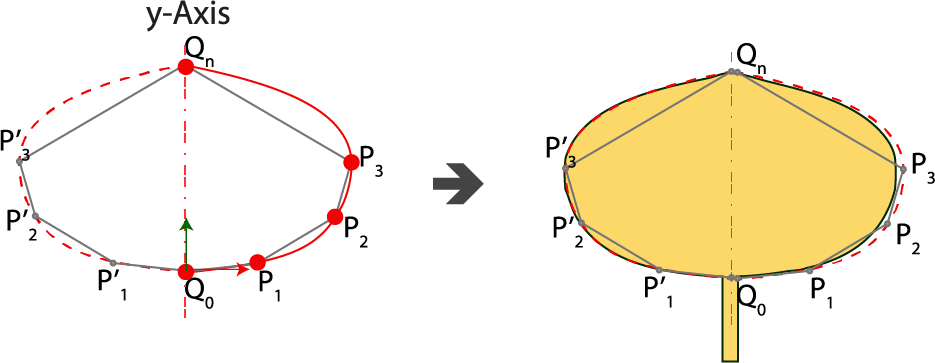
\includegraphics[width=0.95\linewidth]{../../assets/figures/Fig2.png}
\caption{Profile of the spline-based radiating element. The curve's shape is governed by primary control points P1 to P3, optimized by the genetic algorithm. The resulting spline is constructed between on-curve vertices Q0 to Qn.}
\label{fig:splineprofile}
\end{figure}

To model the radiator mathematically, the spline is expressed as a sequence of quadratic segments connecting vertices $\mathbf{Q}_{n-1}$ and $\mathbf{Q}_n$, with each segment controlled by a primary point $\mathbf{P}_n$. A standard quadratic Bézier formulation is used:
\begin{equation}
\mathbf{B}_n(t) = (1-t)^2 \mathbf{Q}_{n-1} + 2t(1-t)\mathbf{P}_n + t^2 \mathbf{Q}_n,\quad t\in[0,1],
\label{eq:bezier_spline}
\end{equation}
where the vertices are often chosen as midpoints between successive control points, i.e., $\mathbf{Q}_n = (\mathbf{P}_n + \mathbf{P}_{n+1})/2$. This representation provides a compact set of geometric degrees of freedom that can be systematically optimized.

The initial antenna configuration is shown in Figure~\ref{fig:antennageom}. The antenna is modeled on a substrate of dimensions $600 \times 600~\mu\text{m}^2$ with thickness $h = 70~\mu\text{m}$. The substrate parameters were selected from the literature and implemented as the material models used in CST and HFSS; frequency-dependent dispersion and solver-specific material-model variations should be considered when reproducing the simulations. The microstrip feed line has width $W_f = 25~\mu\text{m}$ and length $L_f = 105~\mu\text{m}$, and the partial ground plane has length $g_l = 500~\mu\text{m}$. These dimensions define a compact footprint that could support future array or MIMO integration.

\begin{figure}[ht]
\centering
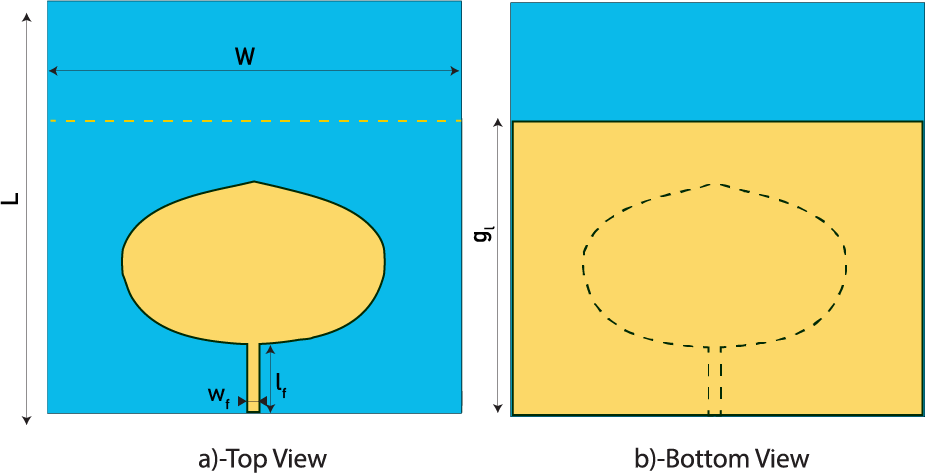
\includegraphics[width=0.9\linewidth]{../../assets/figures/Fig3.png}
\caption{Initial antenna configuration showing the top view with the spline-based radiating element and feed line, and the bottom view with the partial ground plane.}
\label{fig:antennageom}
\end{figure}

The key geometric parameters for the final design are summarized in Table~\ref{tab:geom_params}. These values correspond to the nominal configuration used throughout the subsequent substrate and PBG studies, as well as in the parametric sensitivity analysis.

\begin{table}[ht]
\centering
\caption{Geometric parameters of the proposed antenna (units in $\mu$m).}
\label{tab:geom_params}
\begin{tabular}{@{}lllllll@{}}
\toprule
Parameter & $W$ & $L$ & $g_l$ & $L_f$ & $W_f$ & $h$ \\
\midrule
Value     & 600 & 600 & 500   & 105   & 25    & 70  \\
\bottomrule
\end{tabular}
\end{table}
%----
\subsection{Genetic Algorithm Optimization of the Spline Radiator}
\label{subsec:ga_optimization}

The shape of the spline-based radiator is governed by a set of control points, which define the continuous contour of the patch. While classical approaches rely on fixed rectangular or circular outlines, here the control-point coordinates are directly optimized using a genetic algorithm (GA) to improve impedance matching and overall radiation performance at 0.35~THz~\cite{john_spline_monopole_2007,kerarti_monopole_2016}.

In the proposed framework, the GA operates on a chromosome that encodes the $x$- and $y$-coordinates of the main spline control points $\mathbf{P}_1$, $\mathbf{P}_2$, and $\mathbf{P}_3$ (and their symmetric counterparts), subject to geometric constraints that preserve the substrate aperture and maintain a feed compatible with a nominal 50~$\Omega$ system impedance. Each individual in the population represents one candidate radiator shape; CST is used to evaluate its fitness by computing the simulated S11 level in dB at 0.35~THz and the bandwidth around the operating frequency.

The S11 level in decibels is defined as $S_{11}^{\mathrm{dB}}=20\log_{10}\lvert S_{11}\rvert$. The optimization objective is written in the following minimization form:
\[
F = w_1 S_{11}^{\mathrm{dB}}(0.35~\text{THz}) - w_2 \Delta f_{\text{BW}},
\]
where $\Delta f_{\text{BW}}$ denotes the \(-10\)~dB impedance bandwidth and $w_1$ and $w_2$ are positive normalized weights selected to balance impedance matching and bandwidth. This form favors a more negative S11 level and a larger impedance bandwidth. The GA starts from an initial population of randomly perturbed spline profiles and iteratively applies selection, crossover, and mutation operators until the objective converges.

This GA-driven spline optimization significantly improves the input matching and radiation performance compared to a manually tuned spline or a conventional patch outline. The optimized control-point coordinates are given in Table~\ref{tab:spline_points}, providing a reproducible description of the final radiator shape.

\begin{table}[ht]
\centering
\caption{Optimized spline control-point coordinates for the radiating element.}
\label{tab:spline_points}
\begin{tabular}{@{}lcc@{}}
\toprule
\textbf{Point} & \textbf{$x$-coordinate ($\mu$m)} & \textbf{$y$-coordinate ($\mu$m)} \\
\midrule
$\mathbf{P}_0$ & 0   & 0   \\
$\mathbf{P}_1$ & 90  & 120 \\
$\mathbf{P}_2$ & 180 & 210 \\
$\mathbf{P}_3$ & 260 & 260 \\
$\mathbf{P}_4$ & 300 & 300 \\
\bottomrule
\end{tabular}
\end{table}
%---

\subsection{Substrate Material Selection}
\label{subsec:substrate}

The choice of substrate is critical for antenna performance in the THz regime. To identify suitable materials for the proposed radiator, the antenna is simulated on five representative THz substrate materials with varying relative permittivity and loss tangent: Poly-tetrafluoroethylene (PTFE), fused silica (Quartz), Sapphire (Al$_2$O$_3$), high-resistivity Silicon (HR-Si), and Gallium Arsenide (GaAs). Table~\ref{tab:substrates} summarizes their dielectric properties around 0.35~THz, using representative literature values near 0.35~THz~\cite{hajiyat_antenna_2021}.

\begin{table}[ht]
\centering
\caption{Properties of common substrates for THz antenna design.}
\label{tab:substrates}
\begin{tabular}{@{}lcc@{}}
\toprule
\textbf{Material} & \textbf{Relative permittivity $\varepsilon_r$} & \textbf{Loss tangent $\tan\delta$} \\
\midrule
PTFE (Teflon)              & 2.7  & 0.0002--0.0007 \\
Fused silica (Quartz)      & 3.8  & 0.0001--0.0002 \\
Sapphire (Al$_2$O$_3$)     & 9.4  & 0.0001--0.0003 \\
High-resistivity Silicon   & 11.9 & 0.0001--0.0010 \\
Gallium Arsenide (GaAs)    & 12.9 & 0.0001--0.0006 \\
\bottomrule
\end{tabular}
\end{table}

Figure~\ref{fig:substrates11} shows the simulated S11 level $S_{11}(f)$ in dB for the spline-based antenna on each substrate, indicating that the PTFE model provides the deepest and best-centered resonance near 0.35~THz. The gain comparison in Figure~\ref{fig:substrategain} further supports this choice, indicating that the simulated PTFE model provides the highest gain among the considered materials. Therefore, PTFE is selected as the substrate for balancing impedance matching and radiation performance.

\begin{figure}[ht]
\centering
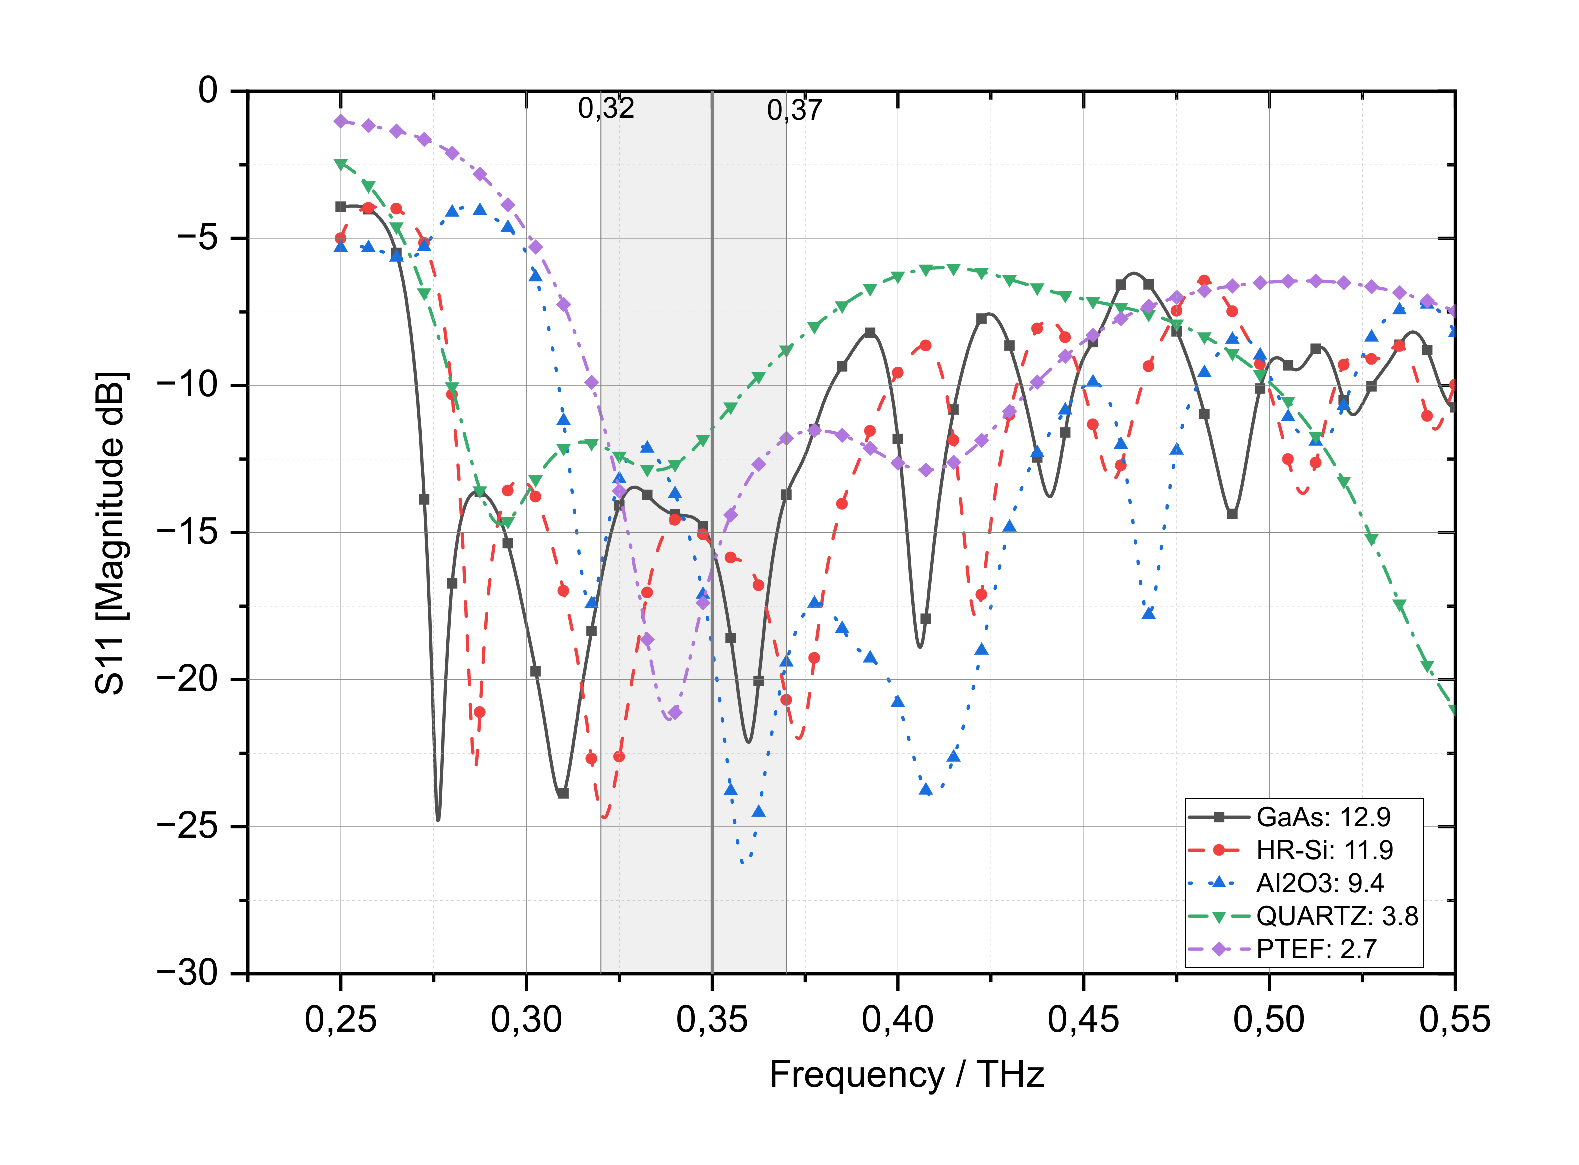
\includegraphics[width=0.99\linewidth]{../../assets/figures/Fig4.eps}
\caption{Simulated S11 level $S_{11}(f)$ in dB for the spline-based antenna on five THz substrate materials; the PTFE model shows the lowest simulated S11 level near 0.35~THz.}
\label{fig:substrates11}
\end{figure}

\begin{figure}[ht]
\centering
\includegraphics[width=0.9\linewidth]{../../assets/figures/Fig5.eps}
\caption{Comparison of the simulated maximum gain in dBi versus frequency for the antenna on five substrate materials; the PTFE model provides the highest gain among the considered cases.}
\label{fig:substrategain}
\end{figure}

The baseline performance of the spline-shaped antenna on the selected PTFE substrate, prior to PBG integration, is summarized in Figure~\ref{fig:ptfegaineff}, which plots maximum gain and radiation efficiency versus frequency.

\begin{figure}[ht]
\centering
\includegraphics[width=0.9\linewidth]{../../assets/figures/Fig6.eps}
\caption{Simulated maximum gain in dBi (left axis) and radiation efficiency (right axis) versus frequency for the spline-shaped antenna on a PTFE substrate (baseline, no PBG).}
\label{fig:ptfegaineff}
\end{figure}

%--new--
\subsection{PBG Structure Design and Integration}
\label{subsec:pbg}

To improve the simulated performance and reduce energy associated with parasitic surface waves, a photonic band-gap (PBG) structure is integrated into the PTFE substrate~\cite{khezzar_pbg_2021,kushwaha_photonic_2018,temmar_bspo_2019}. The PBG lattice consists of a periodic arrangement of cylindrical air holes surrounding the radiating patch, creating a frequency bandgap intended to inhibit surface-wave propagation near the operating frequency and redirect energy toward the main radiating aperture.

As illustrated in Figure~\ref{fig:pbggeom}, the PBG structure is implemented as a 2D square array of air holes embedded in the substrate around the spline-shaped radiator. The holes have radius $r$ and period $p$ in both $x$- and $y$-directions, and span the full substrate thickness $h = 70~\mu\text{m}$, so that the perforation thickness $t_{\mathrm{PBG}}$ is equal to $h$. The array comprises $N_x \times N_y$ cells, and the offset $d_{\mathrm{edge}}$ denotes the nominal minimum distance between the outer spline contour and the nearest hole center. It was fixed in the reported geometry to provide clearance between the metallization and the perforations; it was not included in the parametric sweep.

\begin{figure}[ht]
\centering
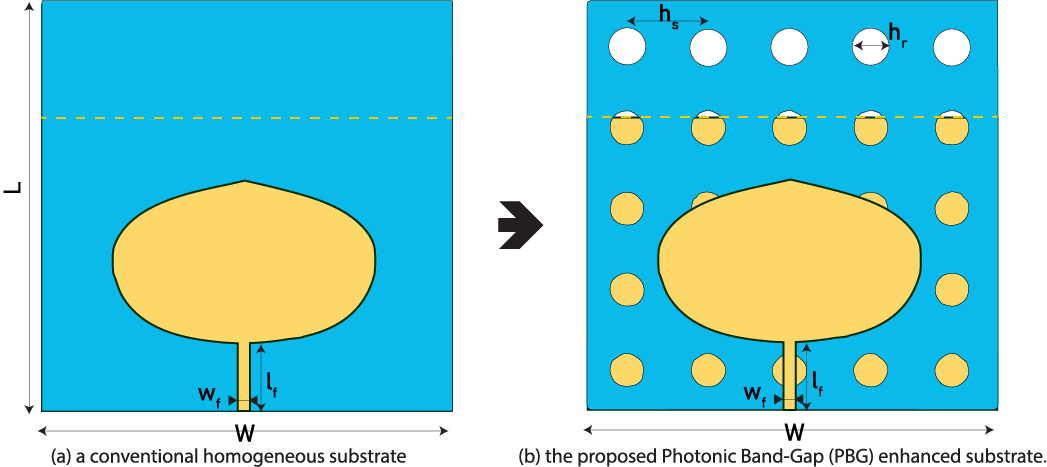
\includegraphics[width=0.9\linewidth]{../../assets/figures/Fig7.png}
\caption{Final antenna geometry on (a) a conventional homogeneous PTFE substrate and (b) the proposed PBG-enhanced PTFE substrate with a periodic lattice of air holes.}
\label{fig:pbggeom}
\end{figure}

The nominal PBG parameters were selected and then evaluated using a unit-cell simulation to determine whether the first stopband was located near 0.35~THz. The resulting transmission response showed reduced transmission around the operating frequency, consistent with suppression of the dominant surface-wave modes. A summary of the PBG geometrical parameters is given in Table~\ref{tab:pbg_params}.

\begin{table}[ht]
\centering
\caption{Geometric parameters of the PBG structure.}
\label{tab:pbg_params}
\begin{tabular}{@{}lcc@{}}
\toprule
\textbf{Parameter} & \textbf{Symbol} & \textbf{Value ($\mu$m)} \\
\midrule
PBG period (in $x$ and $y$)      & $p$              & 123 \\
Hole radius                      & $r$              & 26.46  \\
Perforated thickness             & $t_{\mathrm{PBG}}$ & $h$ \\
Number of cells along $x$        & $N_x$            & 5   \\
Number of cells along $y$        & $N_y$            & 5   \\
Offset from radiator edge        & $d_{\mathrm{edge}}$ & 50 \\
\bottomrule
\end{tabular}
\end{table}

\smallskip\noindent
All PBG air holes are modeled as through-holes, i.e., $t_{\mathrm{PBG}} = h$.

\normalsize
\subsection{Simulation Setup and Cross-Validation}
\label{subsec:sim_setup}

To ensure the reliability of the reported results, two independent full-wave electromagnetic solvers are employed:

\begin{itemize}
  \item \textbf{CST Microwave Studio} --- based on the Finite Integration Technique (FIT), which discretizes Maxwell's equations in integral form on a structured computational grid.
  \item \textbf{ANSYS HFSS} --- based on the Finite Element Method (FEM), which solves the wave equation over tetrahedral mesh elements in the frequency domain.
\end{itemize}

Running both simulations independently and cross-comparing the results mitigates solver-specific numerical artifacts and provides a high level of confidence in the antenna performance. The spline-based radiator and the PBG lattice are implemented with identical geometrical parameters in both solvers, and the same material models are used for the PTFE substrate and the metallization.

To quantify the agreement between the two tools, the relative deviation in resonant frequency and the mean absolute error between the CST and HFSS $\lvert S_{11} \rvert$ responses are evaluated over the operating band. For both the homogeneous and PBG-enhanced configurations, the difference in the resonant frequency remains below 3\% of the nominal 0.35~THz value, while the mean absolute discrepancy in $\lvert S_{11} \rvert$ does not exceed 1.5~dB across the \(-10\)~dB bandwidth. Similar trends are observed for the realized gain curves, with peak-gain variations within 0.3~dB. These results confirm that the proposed antenna exhibits consistent behaviour when analyzed by two distinct numerical techniques, thereby validating the robustness of the design and the conclusions drawn from the simulations.


% III. RESULTS AND ANALYSIS

\section{Results and Analysis}
\label{sec:results}

This section presents the simulated performance of the proposed antenna, comparing the baseline homogeneous PTFE design with the final PBG-enhanced configuration. The results from both CST and HFSS simulations are reported to validate the findings, and the impact of PBG parameters on bandwidth, gain, and efficiency is examined through the parametric sensitivity analysis.

\subsection{Impedance Bandwidth and Return Loss}
\label{subsec:s11_bw}

For the spline-shaped antenna on a homogeneous PTFE substrate (baseline configuration), CST and HFSS simulations produced resonant frequencies near 0.336~THz and 0.346~THz, with corresponding minimum S11 levels of approximately $-23.0$~dB and $-20.4$~dB, respectively. The simulated performance on all five candidate substrates for this baseline configuration is summarized in Figure~\ref{fig:substrates11}, highlighting PTFE as the best choice in terms of matching and centering of the resonance.

The PBG structure changed the simulated matching response. As illustrated in Figure~\ref{fig:pbgs11substrates}, the PBG-enhanced antenna on PTFE exhibits a deeper resonance near the target frequency than the other substrate cases. The comparative plot in Figure~\ref{fig:pbgvsbaselines11} shows an S11 minimum near $-44.65$~dB at 0.35~THz in CST, while HFSS gives a minimum near $-26.3$~dB at a closely aligned resonant frequency. The simulated $-10$~dB impedance bandwidth extends from approximately 0.327 to 0.383~THz, corresponding to about 56~GHz.

\begin{figure}[ht]
\centering
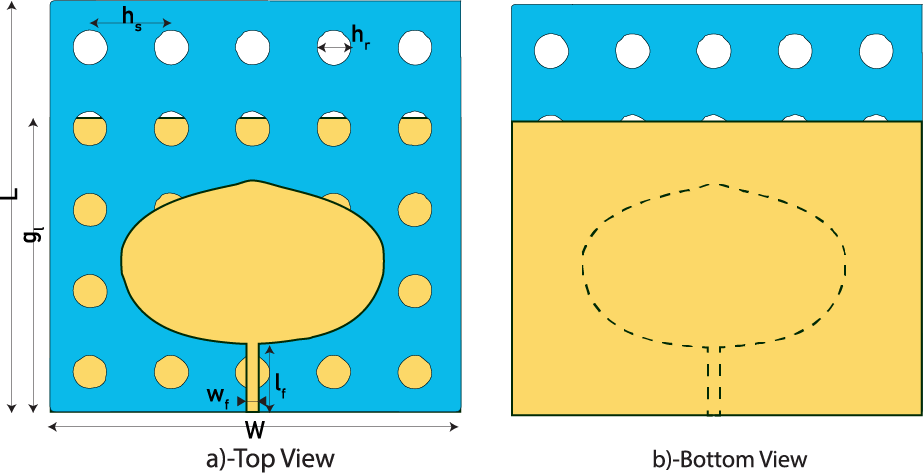
\includegraphics[width=0.9\linewidth]{../../assets/figures/Fig8.png}
\caption{Simulated S11 level $S_{11}(f)$ in dB for the PBG-enhanced antenna on five substrate materials; the curves show the combined effect of substrate permittivity and the PBG structure on impedance matching.}
\label{fig:pbgs11substrates}
\end{figure}

\begin{figure}[ht]
\centering

\includegraphics[width=0.99\linewidth]{../../assets/figures/Fig9.eps}
\caption{Comparison of the simulated S11 level $S_{11}(f)$ in dB for the antenna on homogeneous PTFE and PBG-enhanced PTFE substrates. CST results are shown with solid lines and HFSS results with dashed lines.}
\label{fig:pbgvsbaselines11}
\end{figure}

The change in impedance matching is interpreted as a consequence of the PBG structure modifying the electromagnetic environment around the radiator, which can reduce trapped surface-wave energy and parasitic coupling. The parametric sensitivity analysis in Section~\ref{subsec:parametric_s11} shows how the simulated bandwidth and S11 response change when the hole radius $r$ and lattice period $p$ are varied.

\subsection{Parametric Sensitivity Analysis}
\label{subsec:parametric_s11}
A parametric analysis was conducted to quantify the influence of the PBG lattice geometry on the impedance-matching response of the proposed antenna. Since the PBG is implemented as a periodic array, each parameter was varied globally for all air holes in the lattice, while the remaining antenna dimensions and material properties were kept unchanged. The investigated parameters were the lattice period $p$ and the air-hole radius $r$.

Figure~\ref{fig:parametric_s11}(a) presents the simulated S11 level in dB for different values of the PBG period, namely $p=115$, $119$, $123$, $127$, and $131~\mu\text{m}$. The resonance remains located close to the target frequency of 0.35~THz for all investigated periods. However, the depth of the impedance-matching minimum changes across the sweep. The nominal value $p=123~\mu\text{m}$ provides the deepest minimum, approximately $-42$~dB, and therefore offers the best matching condition at the targeted operating frequency. Period values below or above $123~\mu\text{m}$ result in a shallower return-loss minimum, indicating that the lattice period affects the coupling between the spline radiator and the periodic PBG substrate.

\begin{figure}[ht]
\centering
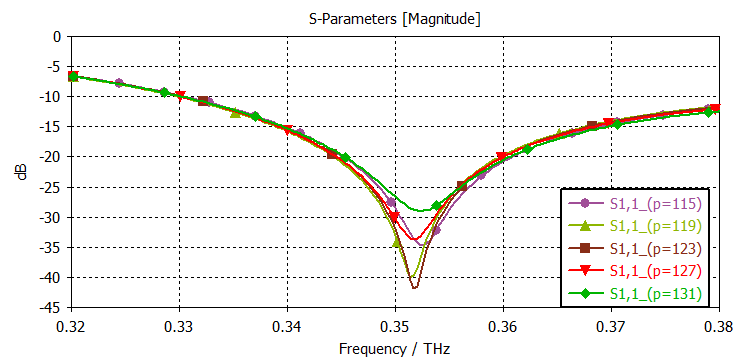
\includegraphics[width=0.9\textwidth]{../../assets/figures/fig_parametric_period_10a.png}\\[2mm]
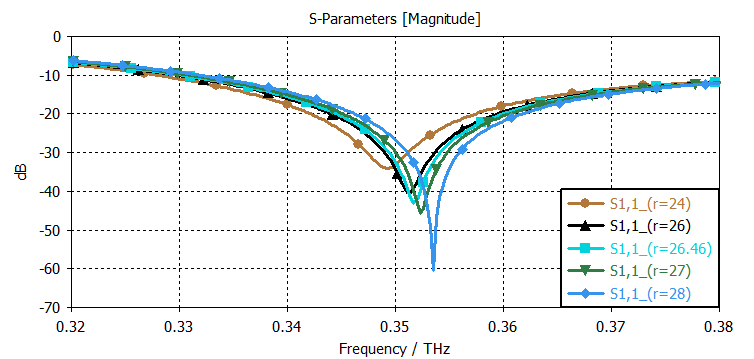
\includegraphics[width=0.9\textwidth]{../../assets/figures/fig_parametric_radius_10b.png}
\caption{Parametric sensitivity of the simulated S11 level in dB for the spline+PBG antenna: (a) effect of the PBG lattice period $p$, with $r=26.46~\mu\text{m}$ fixed; (b) effect of the PBG air-hole radius $r$, with $p=123~\mu\text{m}$ fixed. In each sweep, the corresponding parameter was changed simultaneously for all holes in the periodic PBG array.}
\label{fig:parametric_s11}
\end{figure}
Figure~\ref{fig:parametric_s11}(b) shows the effect of varying the air-hole radius. The investigated values are $r=24$, $26$, $26.46$, $27$, and $28~\mu\text{m}$. Increasing the hole radius causes a progressive shift of the resonance towards higher frequencies. Although some radius values can produce a deeper S11 minimum, their resonances move away from the intended 0.35~THz atmospheric window. The nominal radius $r=26.46~\mu\text{m}$ provides a compromise between a deep simulated S11 minimum and resonance alignment with the target operating frequency. The deepest value observed in this parameter sweep is not used as the final design criterion when its resonance is displaced from 0.35~THz.

The parametric results support the selected PBG geometry. In particular, the final design uses $p=123~\mu\text{m}$ and $r=26.46~\mu\text{m}$, which jointly provide the best impedance matching while preserving resonance operation near 0.35~THz.

\subsection{Gain and Radiation Efficiency}
\label{subsec:gain_eff}

The PBG structure was introduced to improve the radiation characteristics without changing the overall antenna footprint. Figure~\ref{fig:pbg_gain_eff} compares the maximum gain and radiation efficiency of the homogeneous and PBG-enhanced designs on PTFE. In the baseline configuration, the antenna produces a peak gain of approximately 6.7~dBi and a radiation efficiency of approximately 91\%. After integration of the PBG lattice, the peak gain increases to about 7.2~dBi and the radiation efficiency exceeds 93.5\% in the reported simulations. These changes are consistent with reduced surface-wave coupling and increased radiation toward the main lobe.

\begin{figure}[ht]
\centering

\includegraphics[width=0.9\linewidth]{../../assets/figures/Fig10.eps}
\caption{Comparison of simulated maximum gain (dBi) and radiation efficiency (\%) for the antenna on a homogeneous PTFE substrate versus the PBG-enhanced substrate, showing the difference between the two substrate cases.}
\label{fig:pbg_gain_eff}
\end{figure}

The parametric responses in Figure~\ref{fig:parametric_s11} show that the PBG geometry affects the input matching of the proposed antenna. Variations in the lattice period $p$ mainly modify the depth of the S11 minimum while preserving resonance close to the target 0.35~THz band. In contrast, variations in the air-hole radius $r$ produce a more pronounced shift of the resonant frequency towards higher frequencies as the radius increases. The nominal values $p=123~\mu\text{m}$ and $r=26.46~\mu\text{m}$ were selected because they provide a compromise between resonance alignment with the 0.35~THz atmospheric window and a deep S11 minimum.

\subsection{Radiation Pattern Analysis}
\label{subsec:rad_patterns}

The 2D radiation patterns at 0.35~THz are shown in Figure~\ref{fig:fig12} for both the H-plane ($xz$-plane, $\Phi = 90^\circ$) and E-plane ($yz$-plane, $\Theta = 90^\circ$). The PBG-enhanced antenna exhibits a directive main beam in both planes, with the simulated patterns indicating reduced spurious radiation and concentration of energy toward broadside.

At 0.35~THz, the half-power beamwidths are 82.2$^\circ$ in the H-plane and 118$^\circ$ in the E-plane, with side-lobe levels below $-17$~dB and a front-to-back ratio of approximately 2.3~dB. These parameters indicate a compromise between directivity and angular coverage. They may be relevant to short-range THz links, although link-level performance and alignment tolerance were not evaluated in this study.

The 3D radiation pattern in Figure~\ref{fig:fig13} shows the reported peak gain of 7.22~dBi and a broadside radiation characteristic in the simulated result. The combination of the spline-based radiator and PBG-enhanced substrate therefore produces a simulated radiation pattern that may be suitable for point-to-point links near the 0.35~THz atmospheric window~\cite{he_overview_2020,hajiyat_antenna_2021}.

\begin{figure}[ht]
  \centering
  
\includegraphics[width=0.9\linewidth]{../../assets/figures/fig12.png}
  \caption{Simulated 2D radiation patterns of the PBG-enhanced antenna at 0.35~THz: (a) H-plane ($xz$-plane, $\Phi=90^\circ$); (b) E-plane ($yz$-plane, $\Theta=90^\circ$).}
  \label{fig:fig12}
\end{figure}

\begin{figure}[ht]
  \centering
  
\includegraphics[width=0.9\linewidth]{../../assets/figures/fig13.png}
  \caption{Simulated 3D radiation pattern of the PBG-enhanced antenna at 0.35~THz, showing a peak gain of 7.22~dBi.}
  \label{fig:fig13}
\end{figure}

\subsection{PBG Unit-Cell Bandgap Analysis}
\label{subsec:pbg_unitcell}

To characterize the bandgap behaviour of the implemented PBG lattice, a unit-cell transmission analysis was performed in CST Studio Suite using the frequency-domain solver. The unit cell shown in Figure~\ref{fig:pbg_unitcell} consists of a perforated PTFE slab with thickness $h = 70~\mu\text{m}$, period $p = 123~\mu\text{m}$ in both directions, and cylindrical air holes of radius $r = 26.46~\mu\text{m}$, matching the PBG parameters in Table~\ref{tab:pbg_params}. Periodic boundary conditions are applied along the $x$- and $y$-axes, and open boundaries are used in the normal direction.

\begin{figure}[ht]
  \centering
  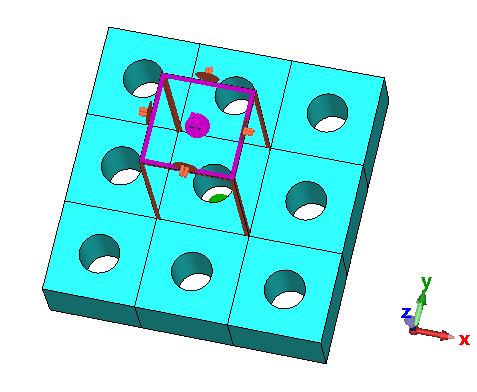
\includegraphics[width=0.9\linewidth]{../../assets/figures/fig14_unitcell.png}
  \caption{Geometry of the PBG unit cell used for bandgap analysis.}
  \label{fig:pbg_unitcell}
\end{figure}

Two Floquet ports are defined on the top and bottom faces of the unit cell, and the S-parameters are evaluated in the range 0.25--0.45~THz. As shown in Figure~\ref{fig:pbg_stopband}, the S21 and S12 traces remain below $-40$~dB and reach minima approaching $-130$~dB, while S11 in dB remains close to 0~dB. The operating frequency of 0.35~THz lies inside this rejecting region, indicating reduced transmission through the unit cell near the operating frequency.

This unit-cell bandgap analysis is consistent with the observed changes in impedance matching, gain, and radiation efficiency after the PBG was integrated beneath the spline-shaped radiating element. The location of the simulated stopband near the target frequency is consistent with reduced surface-wave transmission and with the more concentrated current distribution observed around the radiator~\cite{khezzar_pbg_2021,temmar_bspo_2019}.

\begin{figure}[ht]
  \centering
  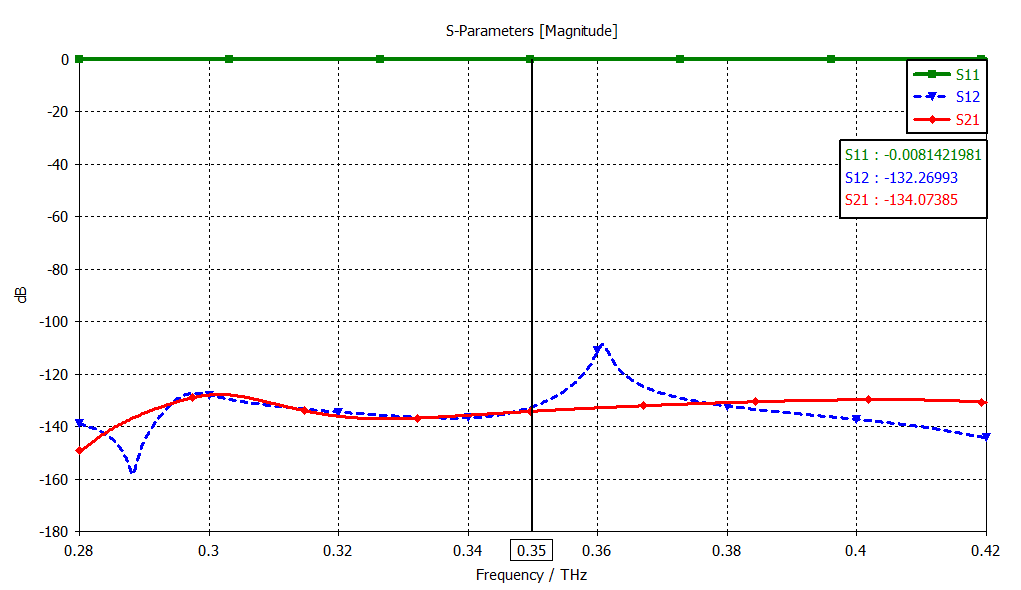
\includegraphics[width=0.9\linewidth]{../../assets/figures/fig15.png}
  \caption{Simulated magnitude of the S-parameters for the PBG unit cell between 0.25 and 0.45~THz.}
  \label{fig:pbg_stopband}
\end{figure}


% IV. DISCUSSION

\section{Discussion}
\label{sec:discussion}
\subsection{Physical Interpretation of Performance Enhancement}
\label{subsec:physical_interpretation}

The simulated performance changes can be interpreted through two complementary mechanisms. First, the continuous curvature of the B-spline geometry produces a smooth surface-current distribution along the radiating element, which may reduce edge diffraction and contribute to the baseline radiation efficiency~\cite{john_spline_monopole_2007,kerarti_monopole_2016}. Second, the periodic air holes of the PBG structure, defined by the parameters in Table~\ref{tab:pbg_params}, create a frequency-specific forbidden band centred near 0.35~THz that is intended to inhibit the propagation of dominant surface-wave modes~\cite{khezzar_pbg_2021,temmar_bspo_2019}.

The simulated surface-current distributions at 0.35~THz further illustrate these trends. For the baseline antenna on homogeneous PTFE, shown in Figure~\ref{fig:baseline_current}, the currents extend along the substrate, indicating surface-wave propagation and edge-related radiation. In contrast, the PBG-enhanced design in Figure~\ref{fig:pbg_current} shows currents that are more concentrated around the spline radiator, with less spreading into the surrounding substrate region. This pattern is consistent with reduced parasitic surface-wave propagation around the radiating aperture.

These mechanisms are consistent with the simulated changes in matching and radiation. The S11 minimum changes from about $-23$~dB for the homogeneous substrate to $-44.65$~dB for the PBG-enhanced configuration. Over the \(-10\)~dB bandwidth, the mean absolute difference between the CST and HFSS S11 curves remains below 1.5~dB, subject to confirmation from the underlying simulation data. The results therefore support further investigation of the spline+PBG antenna for short-range THz links~\cite{strinati_6g_2019,he_overview_2020,hajiyat_antenna_2021}.

\begin{figure}[ht]
  \centering
  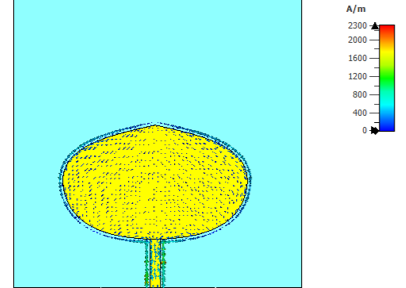
\includegraphics[width=0.9\linewidth]{../../assets/figures/figure_current_noBPG.png}
  \caption{Simulated surface-current distribution on the spline-shaped radiator at 0.35~THz for the baseline antenna on homogeneous PTFE (no PBG).}
  \label{fig:baseline_current}
\end{figure}

\begin{figure}[ht]
  \centering
  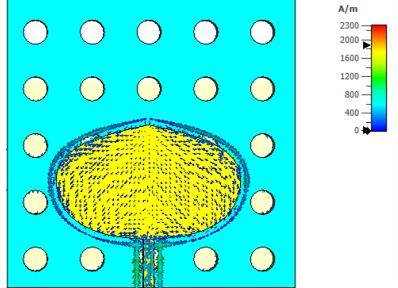
\includegraphics[width=0.9\linewidth]{../../assets/figures/figure_current_BPG.png}
  \caption{Simulated surface-current distribution on the spline-shaped radiator at 0.35~THz for the proposed PBG-enhanced PTFE substrate.}
  \label{fig:pbg_current}
\end{figure}

\subsection{Benchmarking Against Recent THz Antennas}
\label{subsec:benchmarking}

To benchmark the design, its performance is compared with selected THz antennas in Table~\ref{tab3}. The entries are ordered chronologically, and the table distinguishes S11, gain, bandwidth, architecture, and the principal reason for performance differences. Values marked ``NR'' were not inserted because they could not be verified directly from the source or an authoritative publisher record.

Table~\ref{tab3} shows that the proposed antenna is evaluated against designs with substantially different operating bands, feeds, substrates, and PBG architectures. Several studies report higher gain or broader bandwidth, but these values are associated with different design conditions, including tri-band operation, CPW feeding, double-layer PBG structures, composite substrates, or a 1$\times$2 graphene array~\cite{li_triband_2024,babaahmed_hybrid_2025,boujmil_pbg_2025,bouzid_pbg_2025,reguig_pbg_ml_2026}. The Remark column identifies these differences to avoid treating the reported values as strictly like-for-like comparisons. The present design instead targets a single passive element at 0.35~THz and emphasizes the joint use of a GA-optimized spline radiator, a PTFE PBG substrate, and CST/HFSS cross-validation. Its contribution is therefore a balanced single-element design, not a claim that PBG, machine learning, PTFE, or GA optimization is individually new.

\begin{sidewaystable}[p]
\centering
\small
\caption{Chronological comparison of selected THz antennas. S11 is reported in dB; gain is reported in dBi where defined by the source, and ``NR'' denotes an unverified value. Remarks identify major differences in architecture or operating conditions.}
\label{tab3}
\renewcommand{\arraystretch}{1.15}
\setlength{\tabcolsep}{3pt}
\begin{tabular}{@{}M{2.2cm}C{1.35cm}C{1.1cm}C{1.2cm}C{1.1cm}M{2.0cm}M{2.2cm}M{3.0cm}@{}}
\toprule
\textbf{Reference} & \textbf{Band} & \textbf{BW} & \textbf{S11} & \textbf{Gain} & \textbf{Architecture / substrate} & \textbf{Main contribution} & \textbf{Remark} \\
\midrule
\cite{elnawawy_ltcc_2012} (2011) & 0.35~THz & 8.6\% & $-25.6$~dB & 5~dBi & Single patch / Ferro A6M LTCC & Early 0.35~THz LTCC patch & Early single-patch reference. \\
\cite{marouf_bezier_2023} (2023) & 3.1--16~THz & $>135\%$ & $-49.94$~dB & 10~dBi & Bézier monopole / RT5880 & Super-wideband spline-like radiator & Different monopole and substrate. \\
\cite{li_triband_2024} (2024) & 0.360/0.580/0.692~THz & NR & $-31.4/-19.3/-64.1$~dB & 6.28/4.84/7.66~dB & Tri-band patch / polyimide-column PBG on silicon & Tri-band PBG microstrip antenna & Tri-band, not single-band. \\

\cite{babaahmed_hybrid_2025} (2025) & Near 0.35~THz & 36.8~GHz & $-26.1$~dB & 9.4~dBi & Patch / PTFE--SWCNT PBG & ML/GA-optimized PBG patch & Composite substrate; narrower BW. \\
\cite{boujmil_pbg_2025} (2025) & 0.1--1~THz & 870~GHz & $-52$~dB & 12.5~dBi & CPW-fed / double-layer PBG & Slot-free wideband PBG & CPW-fed double-layer architecture. \\
\cite{bouzid_pbg_2025} (2025) & Near 0.65~THz & 32.94~GHz & $-27.64$~dB & 7.36~dB & Patch / 2D cuboid-PBG polyethylene & 2D/3D PBG optimization & Different band, PBG, and substrate. \\
\cite{reguig_pbg_ml_2026} (2026) & 0.3~THz & $\approx23$~GHz & $<-50$~dB & 10.52~dBi & 1$\times$2 graphene patch / hybrid PBG Kapton II & Hybrid PBG with ML prediction & 1$\times$2 array and graphene--PBG hybrid. \\
\midrule
\textbf{This work} & \textbf{0.35~THz} & \textbf{56.42~GHz} & \textbf{\shortstack{$-44.65$~dB CST;\\ $-26.28$~dB HFSS}} & \textbf{7.22~dBi} & \textbf{Single patch / PBG-enhanced PTFE} & \textbf{GA-optimized spline + PBG} & \textbf{Single element; no array gain.} \\
\bottomrule
\end{tabular}
\end{sidewaystable}


\subsection{Sensitivity to Fabrication Tolerances and Prospects}
\label{subsec:tolerances}

Given the micrometer-scale dimensions of the proposed 0.35~THz antenna, fabrication tolerances may affect its performance. In practice, lithography and etching processes on PTFE substrates may introduce variations in hole radius, lattice period, substrate thickness, and metallization edges. The present simulations do not include a statistical tolerance analysis; therefore, the effect of these variations remains to be quantified.

While a full statistical tolerance analysis is left for future work, the simulated geometry may be compatible in principle with established THz micromachining approaches~\cite{he_overview_2020,hajiyat_antenna_2021}. Building on this single-element platform, a natural extension is the development of spline-based PBG arrays and MIMO configurations, where the same principles of surface-wave suppression and smooth current distribution can be exploited to achieve higher directivity, beam shaping, or spatial multiplexing for 6G THz links~\cite{nirob_grid_2025,mousa_ebg_2026}.

Furthermore, recent works on ML- and GA-assisted synthesis of THz antennas and PBG substrates suggest that the proposed spline+PBG framework could be combined with data-driven optimization to explore larger design spaces and accelerate the configuration of future array and MIMO architectures~\cite{babaahmed_hybrid_2025,merino_machine_2025}.



% V. CONCLUSION

\section{Conclusion}
\label{sec:conclusion}

This study presented a compact spline-based microstrip patch antenna operating in the 0.35~THz atmospheric transmission window and modeled on a PTFE substrate. The radiating element was defined by a quadratic spline contour whose control-point coordinates were optimized using a genetic algorithm, yielding a smooth current path and improved input matching compared with conventional rectangular patches. A photonic band-gap lattice of cylindrical air holes was integrated into the substrate, and its first bandgap was centered around 0.35~THz in the unit-cell analysis. The resulting transmission response was consistent with reduced propagation near the operating frequency.

Full-wave simulations using CST Microwave Studio and ANSYS HFSS showed consistent trends between the two solvers. The baseline spline radiator on homogeneous PTFE produced an S11 level of approximately $-23$~dB, a peak gain of 6.74~dBi, and a radiation efficiency of 91.26\%. With the PBG structure, the S11 minimum reached $-44.65$~dB at 0.35~THz in CST and approximately $-26.28$~dB near 0.344~THz in HFSS. The \(-10\)~dB impedance bandwidth was 56.42~GHz, corresponding to approximately 16\% fractional bandwidth, while the peak gain and radiation efficiency increased to 7.22~dBi and 93.56\%, respectively. A unit-cell bandgap analysis of the PBG lattice showed strong transmission suppression in the 0.25--0.45~THz range, and the simulated surface-current distributions showed that the air-hole perforations confined currents around the spline radiator and reduced substrate-wave spreading.

Beyond these quantitative results, the proposed design methodology shows how spline-based GA optimization and PBG substrate engineering can be combined within a single-element architecture. The use of PTFE and cylindrical perforations may be compatible in principle with established micromachining processes for THz devices, while the parametric framework for PBG geometry provides a basis for future tolerance studies and machine-learning-assisted optimization.

Future work will include experimental prototyping of the spline+PBG antenna, including on-wafer measurements of S11, gain, and radiation patterns in the 0.35~THz window. The proposed element also provides a natural building block for spline-based PBG arrays and MIMO configurations, where the principles of surface-wave suppression and smooth current distribution can be exploited to achieve higher directivity, beam shaping, and spatial multiplexing. Combining the present design framework with data-driven and evolutionary optimization techniques may further accelerate the exploration of larger design spaces and support the development of reconfigurable THz antenna architectures for 6G and beyond.




\begin{acknowledgement}
The authors acknowledge the support and collaboration of the research team at the Laboratory of Telecommunications and Information Technologies and the institutional support of the Directorate-General for Scientific Research and Technological Development.
\end{acknowledgement}

\begin{funding}
None declared.
\end{funding}

\begin{conflictofinterest}
The authors declare no conflict of interest.
\end{conflictofinterest}

\section*{Data availability}
The antenna dimensions, material parameters, simulation ranges, and reported numerical results needed to understand the conclusions are provided in the manuscript, tables, and figures. Additional clarification regarding the CST and HFSS model setup is available from the corresponding author upon reasonable request.

\section*{AI disclosure}
Manus AI and OpenAI-based language assistance were used during manuscript preparation in August 2026 for English grammar and clarity editing, organization and restructuring of selected passages, LaTeX formatting support, bibliography consistency checks, and preparation of the cover letter. The tools were not used to generate or modify electromagnetic simulation data, figures, numerical results, CST or HFSS models, scientific analyses, or conclusions. The authors independently checked all AI-assisted text and remain fully responsible for the manuscript.

\bibliographystyle{unsrtnat}
\bibliography{references}
\end{document}
